\chapter{The Standard Model}
\label{ch:the_sm}
    
	The \gls{sm} of particle physics is a quantum field theory that postulates the existence of three generations of quarks and leptons interacting through three fundamental forces: electromagnetic, weak and strong. From the mathematical point of view the \gls{sm} is a gauge quantum field theory that has internal symmetries of the unitary product group $SU(3)\cross SU(2)_L \cross U(1)$.  The fourth fundamental force, namely the gravity, is not included in the \gls{sm}. Nevertheless, since the magnitude of the gravity interaction is negligible on the microscopic scale, it has little to no effect on the precision of the \gls{sm} predictions. The model has 18 free input parameters\footnote{There are \gls{sm} extensions that take into account the non-zero neutrino mass. Then the model gets 7 additional parameters, so their total number reaches 25. Although current thesis only considers the \gls{sm} where neutrinos are massless.} - the physical constants that can not be predicted from within the theory and must be measured experimentally. Evidently, the \gls{sm} predictions are based on these parameters, so the better we know them - the better we can predict how nature behaves on the micro level. The free parameters of the \gls{sm} are briefly described in section \ref{sec::sm_gen}\\

	A comprehensive description of the quantum field theory formalism goes beyond the scope of the current dissertation and can be found in the corresponding textbooks \cite{Peskin}, \cite{bogol}, \cite{Srednicki}, \cite{Berest}, \cite{weinberg}, \cite{Griffiths}. In the following section a brief overview of key \gls{sm} features and constituent parts is provided. \\        
 \section{General composition and key parameters}
 \label{sec::sm_gen}
	In this section I will describe the fields that enter the \gls{sm}. Their existence and interactions result in the three fundamental forces that are taken into account by the theory. The quanta of these fields are also called fundamental particles and possess a number of properties like mass, charge (or charges) and spin (see figure \ref{fig::SMwiki}). The fundamental particles are divided into two groups based on their spin: particles with integer spin are called fermions and those with half-integer spin are bosons. \\
	Let's start from the fermion sector. According to the Pauli exclusion principle\cite{pep} two fermions can not occupy the same quantum numbers. This in turn, has a consequence that the fermions must occupy a finite volume in space-time and as a result make up matter. Half of the fundamental fermions have colour charge and therefore take part in strong interaction - they are called quarks. The other six fermions do not have colour charge and are called leptons (from Greek "$\lambda \epsilon \pi \tau o \sigma$" meaning "little", as they are lighter than the quarks of the same generation). Different types of quarks and leptons are also called flavours, so there are 6 flavours of quarks and 6 flavours of leptons.\\
	For some reason which is yet unknown the twelve elementary fermions make three generations. Particles in the second and third generations have exactly the same charge and spin as the particles of the first generation, but are heavier and also unstable.  Normally the particles of higher generations quickly decay down to their lighter kin of the first generation and can only be observed in cosmic rays and particle accelerators. That means all the matter that surrounds us consists of the four fundamental fermions of the first generation\footnote{Strictly speaking we already know that this is not completely true for the neutrinos, as they oscillate between the flavours due to their tiny mass. But in the \gls{sm} neutrinos are assumed to be massless.}(the first column in Fig. \ref{fig::SMwiki}).\\
	The two quarks of the first generation are called up-quark and down-quark (or u-quark and d-quark for short). All the nuclei of the ordinary matter we see around are built out of these two types of quarks. Quarks are capable of interacting through all three \gls{sm} forces: electromagnetic, weak and strong. Electrons, muons and tau-leptons are sensitive to electromagnetic and weak interaction, while neutrinos can interact (and therefore be detected) only through the weak force. For this reason in particle physics the term "leptons" is sometimes used in a narrow sense referring to electrically charged leptons only. For all quarks and charged leptons the antiparticles were observed as well as the corresponding annihilation phenomena. It is still not clear if neutrinos and antineutrinos of the same flavour are distinct particles.\\
	From our experience we know that matter interacts with matter. But within the \gls{sm} fermions do not interact with each other immediately. The interaction is mediated by boson-type particles. The \gls{sm} includes five types of bosons: four vector bosons serving as force carriers for electromagnetic, weak and strong interactions, and a spinless Higgs boson whose role will be described in more detail in the corresponding subsection \ref{sec::ewk}. The Higgs boson, along with the W and Z bosons are massive, while photons and gluons are massless.\\
	The masses of the fundamental particles make 12 out of 18 free parameters of the \gls{sm}\footnote{The masses of the W and Z bosons can be replaced by other parameters, e.g. weak mixing angle $\theta_W$ and Higgs potential vacuum expectation value (v. e. v.).}. \\
	As it was mentioned, bosons interact with fermions through fundamental interactions. The interaction depends on the charge of the interacting particles and on the type of the interaction itself. Each type of interaction has a coupling constant that defines the scale of the interaction. Hence two more parameters to the \gls{sm}: the strong and electromagnetic coupling constants (the latter is also called the fine structure constant). The weak coupling constant is redundant since it can be obtained from other parameters.\\
	And the remaining four parameters are coming from the \gls{ckm} matrix, that contains information on the strength of the flavour-changing weak interaction~\cite{PhysRevD.86.010001}. 
	
	 \begin{figure}[htpb]
		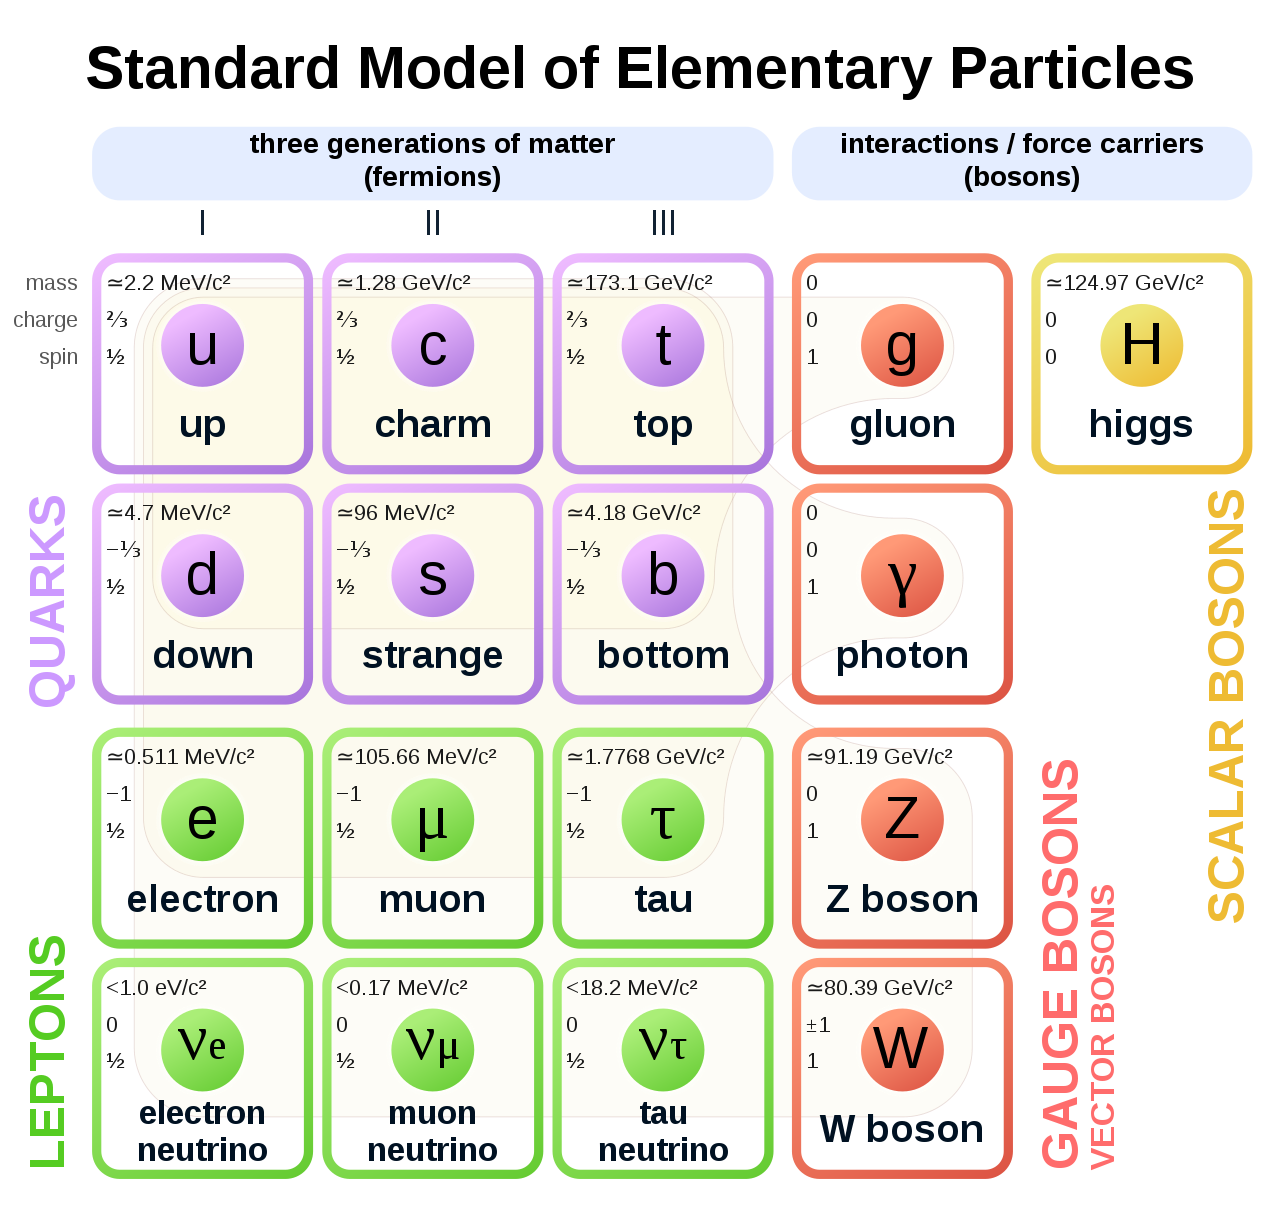
\includegraphics[width=\textwidth,keepaspectratio]{SMwiki.png}
		\caption{The list of particles that enters the \gls{sm}\cite{sm_wiki}. }
		\label{fig::SMwiki}
	\end{figure}
		
An important feature of the \gls{qft} is that particles also interact with physical vacuum. For instance, a charged particle polarizes the physical vacuum, so the vacuum screens the charge of the particle\cite{Schwinger_polariz}.This interaction with virtual particles depends on the energy scale and so do the observed quantities like charge, mass etc. The \gls{sm} is able to predict parameter evolution, so if the value of a certain input parameter $q_0$ is known at the energy $\Lambda_0$ then it is possible to predict its measurable value $q$ at the energy $\Lambda$. This changing of physical parameters is an integral part of the \gls{qft} and is called \textit{renormalisation} \cite{bogol}, \cite{Glashow:1959wxa}. In the Figure \ref{fig::running} the dependence of the inverted \gls{sm} coupling constants on the energy is shown. \\

	 \begin{figure}[htpb]
	 	\centering
	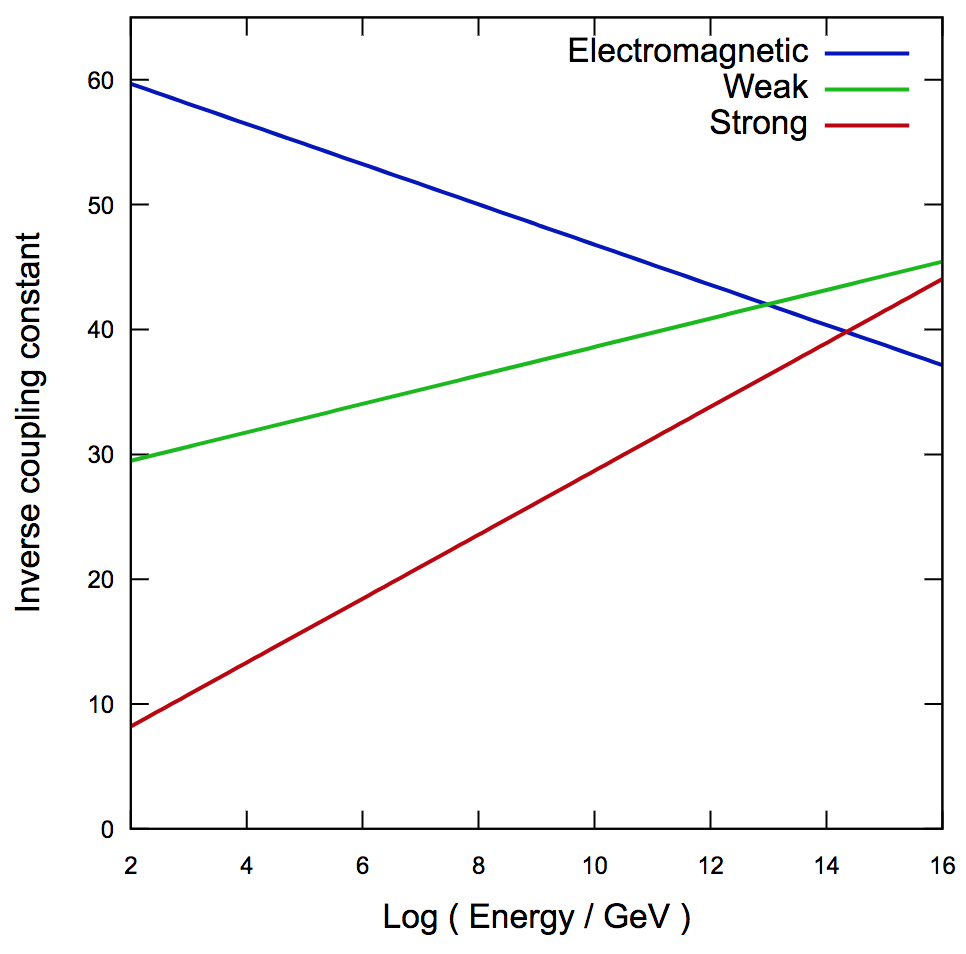
\includegraphics[width=0.6\textwidth,keepaspectratio]{coup_const.png}
	\caption{The running of the inverted \gls{sm} coupling constants \cite{coupl_wiki}. }
	\label{fig::running}
	\end{figure}
As we can see from picture \ref{fig::running} the strong coupling constant is decreasing with the energy. This phenomenon is called \textit{the asymptotic freedom} \cite{Gross}, \cite{Politzer}, \cite{Vanyashin}.



\section{Classical fields and gauge invariance principle}
\label{sec::gauge}
A consistent mathematical description of fields appears to be a more challenging task compared to the description of physical objects that have a definite size and shape even in the classical case. The derivation of Maxwell's equations has been a great success and allowed to obtain the first equations of motion of relativistic fields. It has also subseqently led to the understanding of special relativity \cite{einstein}, \cite{poincare}, \cite{lorentz}. Although for a more general case of fields other than electromagnetic it would be very useful to adopt a more systematic approach like that of Lagrangian or Hamiltonian in classical mechanics. \\
It has turned out that for the relativistic case the Hamiltonian approach was not quite convenient, as the dedicated role of time over other degrees of freedom was in discord with relativistic space-time unification. However it was found possible to describe the fields within the Lagrangian approach. In classic mechanics the action of a mechanical system of $i$ mechanical objects is defined as:
 \begin{equation}
\nonumber
S = \int Ldt = \int \left( \sum_i T_i - U_i \right) dt,
\end{equation}
where $T_i$ and $U_i$ are the kinetic and potential energies of the $i^{th}$ object. Considering that by definition a field exists in every point of space-time, we need to define the Lagrangian density such that $L = \int \mathcal{L}(\phi,\partial_{k}\phi,\dot\phi ) d^3x$, where $\phi$ is a field and $\partial_{k}\phi = \nabla\phi$ - the field gradient, $\partial_{k} = \frac{\partial}{\partial x^{k}}$,  k = 1, 2, 3. Here and further Latin indices run through (1, 2, 3) and are used to denote spatial coordinates, while Greek indices denote space-time coordinates and run though (0, 1, 2, 3). So the action would look like: 
 \begin{equation}
S = \int Ldt =\int \mathcal{L}(\phi,\partial_{\mu}\phi,\dot\phi ) d^4x,
\end{equation}
Now we may use the principle of least action to obtain the equations of motion using the Euler-Lagrange formalism. Let's check it with the example of electromagnetic fields. The Lagrangian density of electromagnetic fields in a vacuum can be written like:
 \begin{equation}
S = -\frac{1}{4}\int F^{\mu \nu}F_{\mu \nu}d^4x.
\end{equation}
The electromagnetic tensor can be defined in terms of electric and magnetic field intensities: $F_{i0}=-F_{0i} = E_i$, $F_{ij} = \epsilon_{ijk}H_k$, where $\epsilon_{ijk}$ is the anti-symmetric Levi-Civita symbol. Alternatively $F_{\mu \nu}$ can be defined in terms of the 4-potential $A_{\mu}$:
 \begin{equation}
F_{\mu \nu} = \partial_{\mu}A_{\nu} - \partial_{\nu}A_{\mu}.
\end{equation}
Now we can safely apply the variational principle, and putting $\delta S=0$ obtain the Maxwell equations in vacuum:
 \begin{equation}
\partial_{\mu}F_{\mu \nu} = 0.
\end{equation}
Noticing the symmetries of the system and using the Noether's theorem\cite{Noether1918} we can find the invariants of electromagnetic field. For example, translational symmetry in time and space ensures conservation of energy and momentum. Let's now consider a symmetry of a different kind. The field potential can be shifted by a gradient of an arbitrary function $\alpha=\alpha(x^\mu)$:

\begin{equation}
\begin{array}{lcl} 
A_{\mu}(x) \rightarrow A^{\prime}_{\mu}(x)  = A_{\mu}(x)+\partial_{\mu}\alpha(x)  \\ 
F_{\mu \nu} \rightarrow F^{\prime}_{\mu \nu}  = \partial_{\mu}(A_{\nu}(x)+\partial_{\nu}\alpha(x))-\partial_{\nu}(A_{\mu}(x)+\partial_{\mu}\alpha(x))=\partial_{\mu}A_{\nu} - \partial_{\nu}A_{\mu}=F_{\mu \nu},
\end{array} 
\end{equation}
where the commutativity of the derivative operator $\partial_{\mu}\partial_{\nu}\alpha(x)=\partial_{\nu}\partial_{\mu}\alpha(x)$ was used.
Let us now consider the electromagnetic theory in the presence of charges and currents:
 \begin{equation}
\mathcal{L} = -\frac{1}{4} F^{\mu \nu}F_{\mu \nu} + j^{\mu}A_{\mu}.
\end{equation}
Now we have an interaction of a field potential $A_{\mu}$ with 4-current $j^{\mu}=(-\rho,j^{i})$. It turns out to be a general property of the field theories: the only form of interaction allowed is between a gauge field and a current.  After applying the gradient field transformation and the least action principle we can obtain the corresponding conservation law:
\begin{equation}
\partial_{\mu}j^{\mu}=0.
\end{equation}
 So this gradient symmetry\cite{bogol} or as it is called more often gauge symmetry leads to the conservation of electric current. If a theory is invariant under gauge transformations then it is called a gauge invariant theory. As we have just seen electrodynamics is the simplest example of such a theory. Taking gauge symmetries into consideration \cite{YangMills} has played a huge role in the development of the \gls{sm}.\\
 Gauge degree of freedom can be constrained in arbitrary way by applying additional conditions on the gauge function. This is called fixing the gauge and becomes necessary after quantization. Any physical result must be gauge-invariant, i.e. must not depend on the gauge. 

\section{Quantum electrodynamics}
\label{sec::qed}
\gls{qed} is a theory of interaction between light and electrically charged particles. Historically it was the first quantum field theory to reach good agreement between quantum mechanics and special relativity. \gls{qed} vacuum has zero expectation value.  Nowadays it is considered to be one of the most precise physical theories ever: theory predictions and experiment results agree up to $~O(10^{-8})$. It has also served as a model for the composition of the subsequent parts of the \gls{sm}, describing other fundamental interactions.\\
Let us consider the free Dirac field based Lagrangian:
 \begin{equation}
\mathcal{L} = \bar \psi(x) (i\slashed\partial - m)\psi(x),
\end{equation}
where $\psi$ and $\bar \psi$ are Dirac wave function and its complex conjugate respectively, $\slashed\partial \equiv \gamma_{\mu}\partial^{\mu}$, $\gamma_{\mu}$ is one of the four gamma-matrices and $m$ is the mass of the Dirac field. 
Such a theory, though, would not be physically consistent. This reflects the fact the quantum nature of spin and spinor fields have to be treated as quantum fields. For instance, an attempt to calculate the energy of a Dirac field would lead to a contradiction: the energy would not be positively defined, as some spinors would have negative energies. \\
This Lagrangian has an internal symmetry to the U(1) transformation: $\psi\rightarrow e^{-i\alpha(x)}\psi$, \: $\bar\psi\rightarrow e^{i\alpha(x)}\bar\psi$. According to Noether's theorem this symmetry implies current conservation: $j^{\mu}=\bar\psi\gamma^{\mu}\psi$.
Now let's get the combined Lagrangian of electromagnetic and Dirac fields, adding the interaction term:
 \begin{equation}
\mathcal{L} = \mathcal{L}_{Dirac^{free}} + \mathcal{L}_{EM^{free}} + \mathcal{L}_{Interaction} = -\frac{1}{4} F^{\mu \nu}F_{\mu \nu}+\bar \psi(x) (i\slashed\partial -m)\psi(x) - q\bar\psi\gamma^{\mu}A_{\mu}\psi,
\end{equation}
where q represents the elementary electric charge. This Lagrangian above is gauge invariant and can be rewritten in a more convenient form:
 \begin{equation}
\mathcal{L} =  -\frac{1}{4} F^{\mu \nu}F_{\mu \nu}+\bar \psi(x) (i\slashed D -m)\psi(x),
\end{equation}
where $D_{\mu} = \partial_{\mu}-iqA_{\mu}$ is a covariant derivative. If one considers space-time in the presence of a field as curved, then $A_{\mu}$ would play a role of connectivity. It must be noted that values like $m$ and $q$ meaning electron mass and charge\footnote{Charge of the electron is related to the electromagnetic coupling constant.} are the \gls{sm} input parameters mentioned in \ref{sec::sm_gen}.  \\
Further calculations are to be performed by the means of the quantum field theory formalism that treats interaction terms like a perturbation to the free fields, making power series expansion in the coupling constant. In the case of electrodynamics the coupling constant is quite small so good precision is reached soon. Since the photons do not directly interact with other photons, \gls{qed} allows only one type of vertex - with two electron lines and one photon line. \\
\begin{figure}
\label{fig::qed}
\centering
\feynmandiagram [horizontal=a to b, baseline=(current bounding box.center)] {
	i1 -- [fermion] a -- [photon] i2,
	a -- [fermion] b,
	f1 -- [photon] b -- [fermion] f2,
};
\feynmandiagram [horizontal=a to b, layered layout] {
	i1 -- [fermion] a,
	a -- [photon, half left] b,
	a -- [fermion] b,
	b -- [fermion] f1,
};
\feynmandiagram [horizontal=a to b,  layered layout, baseline=(b)] {
	i1 -- [photon] a,
	a -- [fermion, half left] b,
	b -- [fermion, half left] a,
	b -- [photon] f1,
};
\caption{Examples of QED diagrams: Compton scattering, electron self-energy, photon self-energy.}
\end{figure}
Although the tree-level processes and diagrams were well understood by 1930th, the loop diagrams were properly explained only by the end of the 1940th making it possible to obtain numerical results of the higher orders of power series expansion and achieve higher precision predictions for QED processes~\cite{Schwinger_covar}, \cite{Schwinger_polariz}, \cite{Feynman_math}, \cite{Feynman_positrons}, \cite{Feynman_spacetime}, \cite{Tomonaga}, \cite{Dyson_all}, \cite{Dyson_smatr}. The examples of QED diagrams are presented in Fig. \ref{fig::qed}.\\
It must be noted that although immediate photon-photon interaction is impossible, light-by-light scattering is still possible through loops:\\

\begin{center}
\feynmandiagram[layered layout, horizontal=a to b] {
	% Draw the top and bottom lines
	i1 
	-- [photon, edge label = \( \gamma \)] a
	-- [fermion, edge label=\(e \)] b
	-- [photon, edge label=\( \gamma \)] f1 ,
	i2 
	-- [photon, edge label=\( \gamma \)]  c
	-- [anti fermion, edge label=\(e \)]  d
	-- [photon, edge label=\( \gamma \)]  f2,
	%Draw the two internal fermion lines
	{ [same layer] a -- [anti fermion, edge label =\(e\)] c },
	{ [same layer] b -- [fermion, edge label=\(e\)] d},
};\\
\end{center}
This process was theoretically described in 1936~\cite{lbl_th} and experimentally observed 83 years after in heavy ion collisions at the LHC \cite{lbl_exp}.
\section{Electroweak theory and the Higgs mechanism}
All the fermions of the standard model are subject to the weak interaction, so its importance for physical processes can not be underestimated. At low energy the weak interaction manifests itself mainly through flavour-changing decays like beta-decay and muon decay. The electroweak theory was created in the end of 1950s~\cite{Glashow:1959wxa} \cite{weinberg} \cite{Salam1959} thanks to numerous experimental results that allowed to shape its properties. The theory assumed that the electromagnetic and weak fundamental forces are actually manifestation of the same field that has a gauge symmetry $SU(2)_L \cross U(1)$ with massive charged and neutral bosons. A few years later the structure of electroweak vacuum was explained along with the mechanism that has allowed the bosons to gain mass \cite{brout}, \cite{higgs}. Assuming this the Lagrangian of the electroweak theory must consist of three parts~\cite{Hollik_2006}: 
\begin{itemize}
	\item Gauge fields that would mediate the interaction.
	\item Fermions that interact with gauge fields
	\item A scalar Higgs field with non-zero vacuum energy that breaks the SU(2) symmetry and couples to the fermions.
\end{itemize}
 \begin{equation}
\mathcal{L}_{EW} = \mathcal{L}_{Gauge} +\mathcal{L}_{Higgs} +\mathcal{L}_{Fermions}
\end{equation}
\subsection{Electroweak gauge fields}
\label{sec::ewk}
As it was already pointed out before, knowing the symmetries of a physical system allows one to compose the gauge fields Lagrangian. The part with U(1) symmetry would look like the electromagnetic field from \ref{sec::gauge} having the hypercharge $Y$, a vector potential $B_{\mu}$ and a gauge coupling $g_1$. The SU(2) field would have 3 vector components $W^{1,2,3}_{\mu}$, three isospin operators $I_1$,$I_2$,$I_3$ and a gauge coupling $g_2$. We can pick the Pauli matrices $\sigma^{i}$ as the representation of generators of the SU(2) group, then the structure constants are $\epsilon_{abc}$ - Levi-Civita symbol.
\begin{equation}
\begin{array}{lcl} 
\mathcal{L_{G}} =  -\frac{1}{4}B_{\mu \nu}B^{\mu \nu} -\frac{1}{4}W^a_{\mu \nu}W^{\mu \nu,a} 
B_{\mu \nu}  =\partial_{\mu}B_{\nu} - \partial_{\nu}B_{\mu}\\ 
W^a_{\mu \nu}  =\partial_{\mu}W_{\nu} - \partial_{\nu}W_{\mu}+g_2\epsilon_{abc}W^b_{\mu}W^c_{\nu},\\ 
\end{array} 
\end{equation}
where the term $g_2\epsilon_{abc}W^b_{\mu}W^c_{\nu}$ appears due to the non-Abelian nature of the SU(2) group (the generators don't commute).


\subsection{Fermion sector}
Each fundamental fermion generation expressed as left-handed doublets and right-handed singlets is a fundamental representation of the group $SU(2) \times U(1)$:

\begin{align}
\begin{pmatrix}
\nu_e  \\
e \\
\end{pmatrix}_L,
\begin{pmatrix}
\nu_{\mu}  \\
\mu \\
\end{pmatrix}_L,
\begin{pmatrix}
\nu_{\tau}  \\
\tau \\
\end{pmatrix}_L,
\begin{pmatrix}
e_R \\
\end{pmatrix},
\begin{pmatrix}
\mu_R \\
\end{pmatrix},
\begin{pmatrix}
\tau_R \\
\end{pmatrix},
\end{align}

\begin{align}
\begin{pmatrix}
u \\
d \\
\end{pmatrix}_L,
\begin{pmatrix}
c  \\
s\\
\end{pmatrix}_L,
\begin{pmatrix}
b\\
t \\
\end{pmatrix}_L,
\begin{pmatrix}
u_R \\
\end{pmatrix},
\begin{pmatrix}
d_R \\
\end{pmatrix},
\begin{pmatrix}
c_R \\
\end{pmatrix},
\begin{pmatrix}
s_R \\
\end{pmatrix},
\begin{pmatrix}
t_R \\
\end{pmatrix},
\begin{pmatrix}
b_R \\
\end{pmatrix}.
\end{align}

Their quantum states are classified using the following quantum numbers: weak isospin $I_3$, $I$, weak hypercharge $Y$. Their electric charge can be obtained using the Gell-Mann-Nishijima relation:
  \begin{equation}
Q = I_3+\frac{Y}{2}.
\end{equation}

The fermions are divided by their chirality: only the left-handed particles take part in weak interaction. The left-handed fermion fields of each lepton and quark generation j
  \begin{equation}
    \psi^L_j = \begin{pmatrix}
	\psi^L_{j+}  \\
	\psi^L_{j-}  \\
\end{pmatrix}
  \end{equation}
make SU(2) doublets, with indices $\sigma=\pm$, while the right-handed fermions can be written as singlets:
 \begin{equation}
\psi^R_j = \psi^L_{j\sigma}.  
\end{equation}
Like in the the electromagnetic case we can define the covariant derivative that would ensure the gauge invariance of the Lagrangian:
 \begin{equation}
D_\mu = \partial_{\mu} - ig_2I_aW^a_{\mu}+ig_1\frac{Y}{2}B_{\mu},
\end{equation}
with $I_a \equiv \frac{\sigma_a}{2}$, then fermion Lagrangian takes the following form:
 \begin{equation}
\mathcal{L}_{Fermions} = \sum_f \bar \psi^L_j i \gamma^{\mu}D_{\mu}\psi^L_j +\sum_{f,\sigma} \bar \psi^R_{f,\sigma}  i \gamma^{\mu}D_{\mu}\psi^R_{f,\sigma}  .
\end{equation}

\subsection{Higgs field breaking the symmetry}
\label{sec:symmetry_breaking}
The Higgs field is represented by single complex a scalar doublet field $\Phi(x)$, that has 4 independent components. It spontaneously breaks the  $SU(2)\times U(1)$ gauge symmetry, leaving the $U(1)_{EM}$ symmetry intact. The Higgs field doublet has the hypercharge $Y=1$:
  \begin{equation}
\Phi(x) = \begin{pmatrix}
\phi^{+}(x)  \\
\phi^{0}(x)  \\
\end{pmatrix}.
\end{equation}
The Higgs field Lagrangian with non-zero vacuum expectation value is: 
 \begin{equation}
\mathcal{L}_{Higgs} = (D_{\mu}\Phi)^+(D_{\mu}\Phi)-V(\Phi)+\mathcal{L}_{Yukawa}.
\end{equation}
The gauge invariance of the Higgs Lagrangian is ensured in the traditional way by using the covariant derivative:
 \begin{equation}
D_{\mu} = \partial_{\mu} - ig_2I_aW^a_{\mu}+i\frac{g_1}{2}B_{\mu}.
\end{equation}
The Higgs potential contains the mass term and quartic self-interaction:
 \begin{equation}
V(\Phi) = -\mu^2 \Phi^+\Phi + \frac{\lambda}{4}\partial_{\mu}(\Phi^+\Phi)^2,
\end{equation}
where $\lambda$ stands for the quartic Higgs self-coupling constant and $\mu$ is the mass of the $\Phi$ field. The vacuum expectation value $<\Phi>$ does not vanish:
  \begin{equation}
<\Phi(x)> = \frac{1}{\sqrt(2)}\begin{pmatrix}
0  \\
v \\
\end{pmatrix},\;\;\;\;\; 
v = \frac{2\mu}{\sqrt(\lambda)}.
\end{equation}
Applying the unitarity gauge \cite{weinberg2} we can constraint three out of four degrees of freedom of the Higgs field and rewrite the Higgs doublet in the following way:
  \begin{equation}
 \Phi(x) = \frac{1}{2}\begin{pmatrix}
 	0 \\
 	v+H(x)  \\
 \end{pmatrix},
  \end{equation}
  which leaves us with a physical real neutral scalar field $H(x)$ with 
    \begin{equation}
	M_H=\sqrt(2)\mu.
  \end{equation}
 This real field would couple to itself forming triple and quartic self-coupling vertices, to the gauge fields through the covariant derivatives and to the charged fermions, giving them mass. The Yukawa term in Lagrangian the unitary gauge is:
     \begin{equation}
\mathcal{L}_{Yukawa}=-\sum_f m_f \bar\psi_f\psi_f-\sum_f \frac{m_f}{v} \bar\psi_f\psi_f H,
 \end{equation}
where
\begin{equation}
m_f=g_f\frac{v}{\sqrt(2)}=\sqrt(2)\frac{g_f}{g_2}M_W.
\end{equation}
The Higgs coupling constants to the corresponding fermion flavour are denoted as $g_f$. This relation between the Higgs coupling and the mass of the W boson illustrates how much the \gls{sm} parameters are intertwined and particularly underlines the importance of the $M_W$ measurement.
\subsection{Physical interpretation of gauge fields and parameters}
The Higgs coupling to the gauge fields results in the following terms in the Lagrangian:
\begin{equation}
\label{eq::weak_basis}
\frac{1}{2}\frac{g_2}{2}v(W_1^2+W^2_2)+\frac{v^2}{4}(W^3_{\mu},B_{\mu}) \begin{pmatrix}
g_2^2  & g_1 g_2 \\
g_1 g_2 & g_1^2   \\
\end{pmatrix}
\begin{pmatrix}
W^3_{\mu} \\
B_{\mu}   \\
\end{pmatrix}.
\end{equation}
In order to get the physical meaning of this expression let us make a transition to the basis of physical fields:
\begin{equation}
\begin{array}{lcl} 
W^{\pm}_{\mu}  &=& \frac{1}{\sqrt{2}}(W^{\mp}_{\mu}\mp iW^{\mp}_{\mu})\\ 
\begin{pmatrix} Z_{\mu} \\ A_{\mu}   \\ \end{pmatrix}  &=& \begin{pmatrix} \cos{\theta_{W}} & \sin{\theta_{W}}\\ -\sin{\theta_{W}}& cos{\theta_{W}}   \\ \end{pmatrix} \begin{pmatrix} W^3_{\mu} \\ B_{\mu}   \\ \end{pmatrix},
\end{array} 
\end{equation}
where $\theta_{W}$ is called the weak mixing angle or the Weinberg angle. In the new basis expression \ref{eq::weak_basis} has transparent physical sense:
\begin{equation}
M^2_W W^+_{\mu}W^{-\mu} +\frac{1}{2} (A_{\mu},Z_{\mu})\begin{pmatrix}
0 & 0 \\
0 & M^2_Z   \\
\end{pmatrix}
\begin{pmatrix}
A_{\mu} \\
Z_{\mu}   \\
\end{pmatrix},
\end{equation}
with
\begin{equation}
\begin{array}{lll} 
M_W &= & \frac{1}{2} g_2 v\\ 
M_Z &=& \frac{1}{2} \sqrt{g_1^2+g_2^2} v.
\end{array} 
\end{equation}
The mixing angle $\theta_W$ also has a very clear physical meaning:
\begin{equation}
\cos{\theta_W}=\frac{g_2}{g_1^2+g_2^2}=\frac{M_W}{M_Z}.
\end{equation}
With $A_{\mu}$ having a sense of electromagnetic potential its coupling to the electron must have a physical meaning of the electric charge $e=\sqrt{4\pi\alpha}$ we can express $e$ in terms of gauge couplings:
\begin{equation}
e=\frac{g_1 g_2}{g_1^2+g_2^2}, \;\;\;\;g_2=\frac{e}{\sin{\theta_W}},\;g_1=\frac{e}{\cos{\theta_W}} .
\end{equation}
Thus the demonstrated Weinberg rotation (see Fig. \ref{fig::weiberg_rotation}) fully replaces the original parameters $g_1$, $g_2$, $\lambda$, $\mu^2$, $g_f$ by another set of measurable values $e$, $M_W$, $M_Z$, $M_H$, $m_f$ which are the input parameters of the \gls{sm}.


\begin{figure}[htpb]
	\centering
	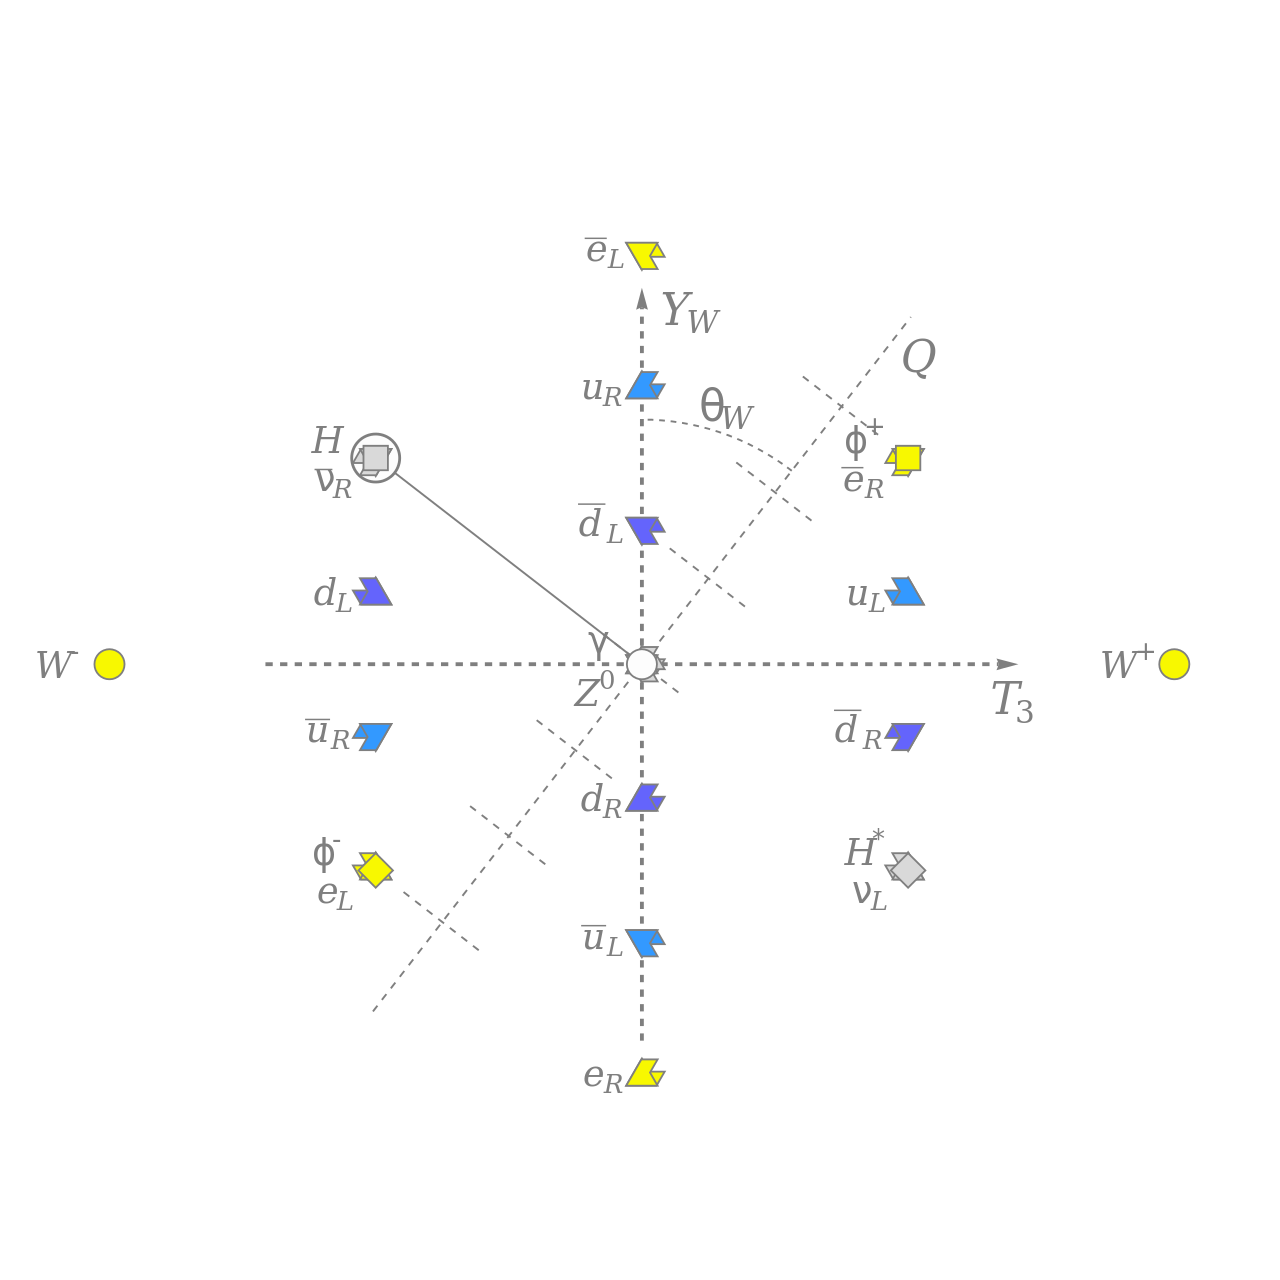
\includegraphics[width=0.65\textwidth,keepaspectratio]{weinb.png}
	\caption{Electroweak sector and the Weinberg rotation \cite{coupl_wiki}. }
	\label{fig::weiberg_rotation}
\end{figure}

\section{Chromodynamics}
\gls{qcd} is a non-Abelian gauge theory that describes strong interaction. \gls{qcd} is symmetric under unbroken SU(3) colour symmetry, so the interaction scheme is built in the same way as electromagnetic and electroweak theories. To preserve the gauge invariance the gauge field of gluons is introduced with 8 components, since SU(N) group has $\frac{N^2-1}{2}$ independent elements. The gluons are massless vector bosons like the photons, although because of the non-Abelian nature of the gauge group they couple not only to the fermions but also to the other gluons. The gauge invariant QCD Lagrangian with kinetic term containing covariant derivative would look like:
\begin{equation}
\begin{array}{lll} 
	\mathcal{L}_{QCD} &=& -\frac{1}{4}F^a_{\mu\nu}F_a^{\mu\nu} + \bar\psi_a(i(\gamma^{\mu}D_{\mu})^{ab} - m\delta^{ab})\psi_b,\\
	F^a_{\mu\nu}  &=& \partial_{\mu}A_{\nu}^a-\partial_{\nu}A^a_{\mu}+g_sf^{abc}A^b_{\mu}A^c_{\nu},\\
	D_{\mu} &=& \partial_{\mu} + ig_s A_{\mu}^at_a.
\end{array} 
\end{equation}
with $\psi$ being the quark field, m is the mass of the quark, a,b = 1, 2, ..., 8 are the colour indices, $g_s$ is the strong coupling constant, $f^{abc}$ are the structure constants of the SU(3) group and $t_a$ are the generators of the SU(3) group. \\
As it was already mentioned in \ref{sec::qed} quantitative calculations in \gls{qft} treat particle interaction as a perturbation to the free field theory. The coupling constant is considered to be a small parameter so every next power of the coupling constant is much smaller than the previous one. Due to asymptotic freedom the constant $\alpha_s$ becomes small at higher energies and allows perturbative calculations. But at a certain energy scale called $\Lambda_{QCD}\approx200$ MeV, \gls{qcd} becomes non-perturbative. It means we may no longer assume that interaction is a small perturbation of the free fields. This phenomenon is known as the \textit{colour confinement}.\\


	 \begin{figure}[htpb]
	 	\centering
	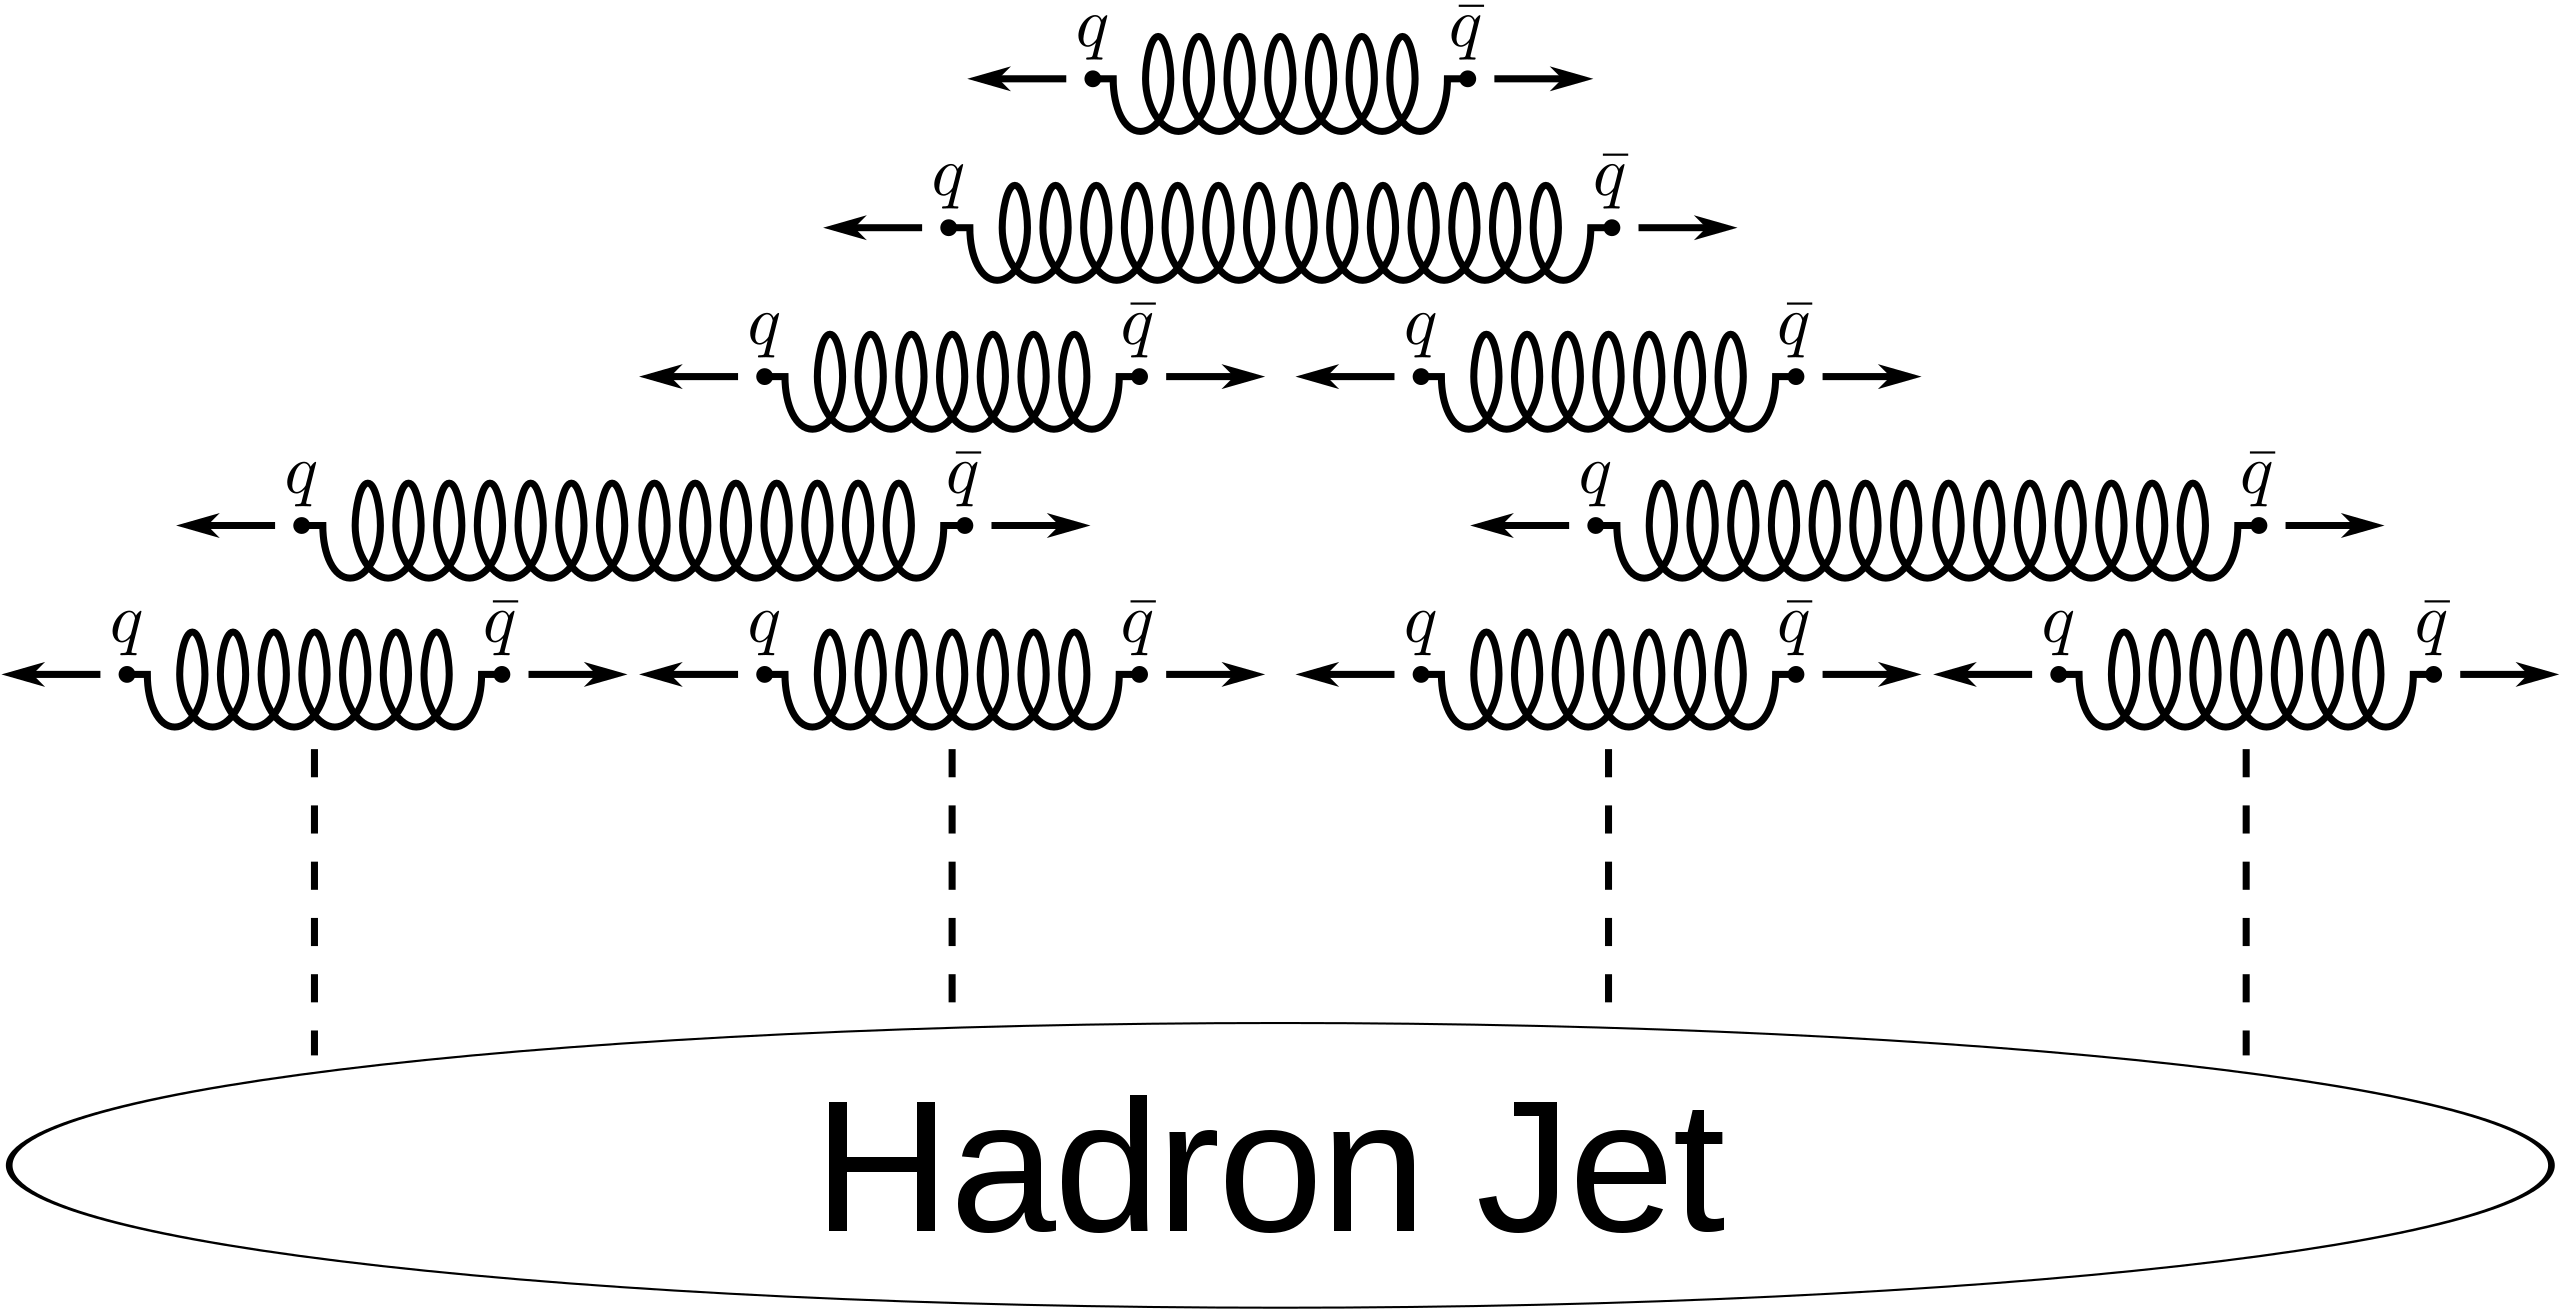
\includegraphics[width=0.75\textwidth,keepaspectratio]{confinement.png}
	\caption{The formation of a hadron jet \cite{conf_wiki}. }
	\label{fig::jet}
	\end{figure}
Because of colour confinement we can only observe colourless objects like baryons and mesons, but not quarks and gluons. If a high-energetic parton gets torn out of a hadron then it creates an avalanche-like process creating quark-antiquark pairs until it fully hadronizes (see Fig. \ref{fig::jet}) confining its colour. Such an avalanche is called a hadronic jet. \\
Currently there is no viable physical theory that would describe \gls{qcd} vacuum and low-energy behaviour of quarks and gluons. This also means that although nuclear forces are evidently residuals of the QCD interaction of partons within the baryons, there is no continuity between \gls{qcd} and nuclear physics. Confinement and low-energy \gls{qcd} remain an unsolved problem of modern physics. 


